\documentclass[11pt]{article}

\usepackage[margin=1in]{geometry}
\usepackage{amsmath, amssymb}
\usepackage{booktabs}
\usepackage{enumitem}
\usepackage{graphicx}
\usepackage{hyperref}
\usepackage{tabularx}
\usepackage{xcolor}
\graphicspath{{figures/}}

\title{Kinematic Classifier Methodology: Automated Study Design, Corpus Synthesis, and Evidence-Grounded Promotion}
\author{kinematic-classifier-sandbox}
\date{\today}

\begin{document}

\maketitle

\begin{abstract}
This document is the cohesive entry point for the repository's methodology track. It collects the corpus, feature, evidence, posterior, evaluation, promotion, and dimensional-lift stories into one narrative so the project can be read as a reusable study system rather than a pile of adjacent 1D experiments. The current 1D witness problems are treated as proofs of methodology layers, not as the final endpoint of the project.
\end{abstract}

\section{How To Read This Paper}
This paper is intentionally a synthesis document rather than a full derivation dump. It should answer five questions in one pass:
\begin{enumerate}[leftmargin=1.5em]
  \item What problem is the repository solving?
  \item What are the reusable layers?
  \item How do corpus, feature, classifier, and posterior machinery fit together?
  \item What evidence is used to promote or reject studies?
  \item What remains to be proved before 3D or advanced filters are justified?
\end{enumerate}

\section{Companion Deep-Dive Documents}
The implementation-linked derivations live in the survey stack. This paper integrates them at the architectural level:
\begin{itemize}
  \item \texttt{posterior\_update\_math} for recursive inference mechanics and walkthrough artifacts,
  \item \texttt{methodology\_evaluation\_framework} for priors, AUC, confusion, PCA, adequacy, and leakage methodology,
  \item \texttt{classifier\_ladder\_and\_contracts} for the pointwise/windowed/accumulator/Kalman/transition ladder and shared contracts,
  \item \texttt{corpus\_generation\_and\_search} for trajectory generation, corpus search, and candidate promotion logic,
  \item \texttt{dimensional\_lift\_and\_advanced\_filter\_gates} for 3D-readiness auditing and IMM/PF/RBPF decision gates.
\end{itemize}

\section{Problem Formulation}
The active repository goal is not only to maximize one benchmark score, but to prove that a study candidate can be declared, screened, executed, audited, and promoted through a reusable methodology surface. A study candidate combines a corpus, feature set, class set, classifier family, prior specification, and optional filtering backend.

\section{Global Methodology Flow}
The repository is best understood as one compositional flow rather than separate notebooks. In compact form,
\begin{align}
\text{corpus objectives}
&\rightarrow
\text{generated corpus}
\rightarrow
\text{feature table and evidence streams}
\notag \\
&\rightarrow
\text{posterior histories}
\rightarrow
\text{evaluation and adequacy artifacts}
\notag \\
&\rightarrow
\text{study candidate}
\rightarrow
\text{validation ladder}
\rightarrow
\text{promote / revise / reject / defer}.
\end{align}
This is the central claim of the repository: classifiers, filters, and feature families are valuable insofar as they can plug into this shared flow without rewriting the downstream evaluation and reporting machinery.

\section{Shared Objects And Notation}
The main reusable objects are:
\begin{itemize}[leftmargin=1.5em]
  \item \(\tau\): one generated trajectory or observation sequence,
  \item \(\mathcal{D}\): a corpus candidate,
  \item \(\phi_t\): feature vector or evidence summary at time \(t\),
  \item \(L_t(c)\): class-conditioned evidence or likelihood term for class \(c\),
  \item \(p_t(c)\): posterior probability of class \(c\) after observing data up to time \(t\),
  \item \(Q_{\text{static}}\): study-candidate screening score before Monte Carlo evidence,
  \item \(Q_{\text{mc}}\): study-candidate confirmation score after executed common-study evidence,
  \item \(d\): terminal decision, with \(d \in \{\texttt{promote}, \texttt{revise}, \texttt{reject}, \texttt{defer}\}\).
\end{itemize}

\section{Generic Study Object}
The machine-readable study candidate schema and validation-ladder schema are implemented in the repository and exercised by the current artifact generation path. The workflow is checklist-driven: static compatibility, corpus adequacy, feature separability, oracle separability, classifier performance, posterior quality, prior sensitivity, robustness, dimensional transfer, and final promotion decision.
In abstract form, a study candidate is a tuple
\begin{equation}
s = (\mathcal{D}, f, \mathcal{C}, m, \pi, b),
\end{equation}
where \(\mathcal{D}\) is a corpus, \(f\) is a feature set, \(\mathcal{C}\) is a class set or class pair, \(m\) is a classifier family, \(\pi\) is a prior regime, and \(b\) is an optional backend or filter family. The validation ladder then maps
\begin{equation}
s \rightarrow \{\ell_1, \ell_2, \dots, \ell_n\} \rightarrow d.
\end{equation}
This means the repo is not just running benchmarks. It is trying to prove that a declared study object can be audited in a standard way.

\section{Bayesian Evidence Model}
The repository treats posterior updating as a reusable contract. For class label $c$ and observation history $y_{1:k}$, the recursive update is
\begin{equation}
p_k(c) = \frac{p(y_k \mid c)\, p_{k-1}(c)}{\sum_{c'} p(y_k \mid c')\, p_{k-1}(c')}.
\end{equation}
In log form,
\begin{equation}
\log p_k(c) = \log p_{k-1}(c) + \log p(y_k \mid c) - \log Z_k,
\end{equation}
and in the two-class case the log-odds recursion becomes
\begin{equation}
\log \frac{p_k(a)}{p_k(b)} = \log \frac{p_{k-1}(a)}{p_{k-1}(b)} + \log \frac{p(y_k \mid a)}{p(y_k \mid b)}.
\end{equation}
This is why the walkthrough artifacts emphasize Bayes factors, prior sweeps, and flip thresholds rather than only endpoint accuracy. The crucial architectural point is that pointwise baselines, windowed summaries, sequential accumulators, Kalman innovation banks, and transition-aware models are all different ways of supplying the class-conditioned evidence term \(p(y_k \mid c)\) or its log form.

\section{Feature Taxonomy}
The methodology distinguishes instantaneous, windowed, cumulative, robust-summary, derivative-based, and model-residual evidence. Instantaneous features look the most like fresh evidence. Windowed and robust features are summary evidence. Cumulative features can double-count prior signal if they are treated as independent measurements. Model-residual features compare observations against class-conditioned dynamics and are therefore the natural bridge toward filtering backends.
If \(\phi(\tau)\) denotes a feature extractor applied to trajectory \(\tau\), then the feature layer is not only a convenience transformation. It defines the evidence geometry that later AUC, overlap, PCA, and separability studies inspect.

\section{Witness Problems}
The repository uses small 1D witness problems as methodological proofs. Their purpose is to isolate one layer of reasoning at a time rather than to claim a finished deployment-grade taxonomy.
\begin{table}[htbp]
\centering
\caption{Witness problems used to prove distinct methodology layers.}
\label{tab:witness_problems}
\begin{tabularx}{\textwidth}{lXXX}
\toprule
toy\_problem\_id & purpose & what\_it\_proves & known\_limitations \\
\midrule
pointwise\_easy\_overlap & Lower-bound instantaneous classifier baseline & A minimal likelihood-only baseline exists and can be audited for prior fragility. & Cannot exploit history or dynamics. \\
windowed\_outlier\_witness & Show robust extrema beating raw extrema under outliers & Feature design changes class stability under corrupted observations. & Feature contributions are not independent Bayes terms. \\
sequential\_history\_help & Demonstrate that sequential accumulation improves over pointwise evidence & History can improve classification and exposes prior sensitivity explicitly. & Still static-class unless switching logic is added. \\
kalman\_endpoint\_match & Show model-based filtering on matched-endpoint irregular tracks & Dynamics-aware evidence helps when endpoint-only reasoning fails. & Position-only sensing remains weak on short noisy horizons. \\
transition\_switching\_bridge & Bridge from static accumulation to explicit switching dynamics & Switching structure can help before IMM is justified. & Not yet a full IMM or nonlinear filter. \\
\bottomrule
\end{tabularx}
\end{table}

\section{Algorithm Ladder}
The classifier ladder is the main experimental spine. Each rung adds one capability and is supposed to address one previously identified failure mode rather than add complexity for its own sake.
\begin{table}[htbp]
\centering
\caption{Algorithm ladder proof summary.}
\label{tab:algorithm_ladder}
\begin{tabularx}{\textwidth}{clXXc}
\toprule
level & algorithm & new\_capability & failure\_mode\_addressed & promotion\_status \\
\midrule
1 & pointwise & Instantaneous class likelihood baseline & No baseline for ambiguity & promote \\
2 & windowed & History-derived engineered features & Pointwise noise sensitivity & revise \\
3 & sequential\_bayes & Recursive posterior accumulation & History ignored by pointwise baseline & promote \\
4 & kalman\_bank & Model-based innovation evidence & Endpoint ambiguity under irregular timing & reject \\
5 & transition\_matrix & Explicit mode switching before IMM & Static accumulator under switching trajectories & pass \\
6 & imm & Switching-aware state mixing with shared posterior output & Transition-only switching evidence saturates & defer \\
7 & particle\_filter\_bank & Sampled nonlinear and non-Gaussian state evidence & Single-Gaussian projections collapse multimodal posterior structure or miss mean-reverting stochastic dynamics & promote \\
8 & rbpf & Sampled latent mode path with conditional analytic state filtering & Pure PF wastes structure on mixed discrete/continuous latent problems & promote \\
\bottomrule
\end{tabularx}
\end{table}

\section{Bayesian Update Walkthrough}
The current repository emits representative Bayesian walkthroughs from promoted and revised study candidates. These use real common-study trajectories and expose prior odds, class-score increments, posterior odds, prior sweeps, and flip thresholds. The step table below is a compact numeric witness of that process.
\begin{table}[htbp]
\centering
\caption{Representative Bayesian walkthrough steps from a promoted study candidate.}
\label{tab:bayes_walkthrough}
\begin{tabularx}{\textwidth}{cccclc}
\toprule
$t_k$ & $p_{k-1}(a)$ & $\Delta \lambda_k^{ab}$ & $p_k(a)$ & $\hat{c}_k$ & $\max_c p_k(c)$ \\
\midrule
0.0 & 0.5 & 0.0 & 0.5 & constant\_velocity & 0.5 \\
0.5 & 0.5 & 0.007 & 0.502 & constant\_velocity & 0.502 \\
1.0 & 0.502 & 0.172 & 0.545 & constant\_velocity & 0.545 \\
1.5 & 0.545 & 0.522 & 0.668 & constant\_velocity & 0.668 \\
\bottomrule
\end{tabularx}
\end{table}

\begin{figure}[htbp]
\centering
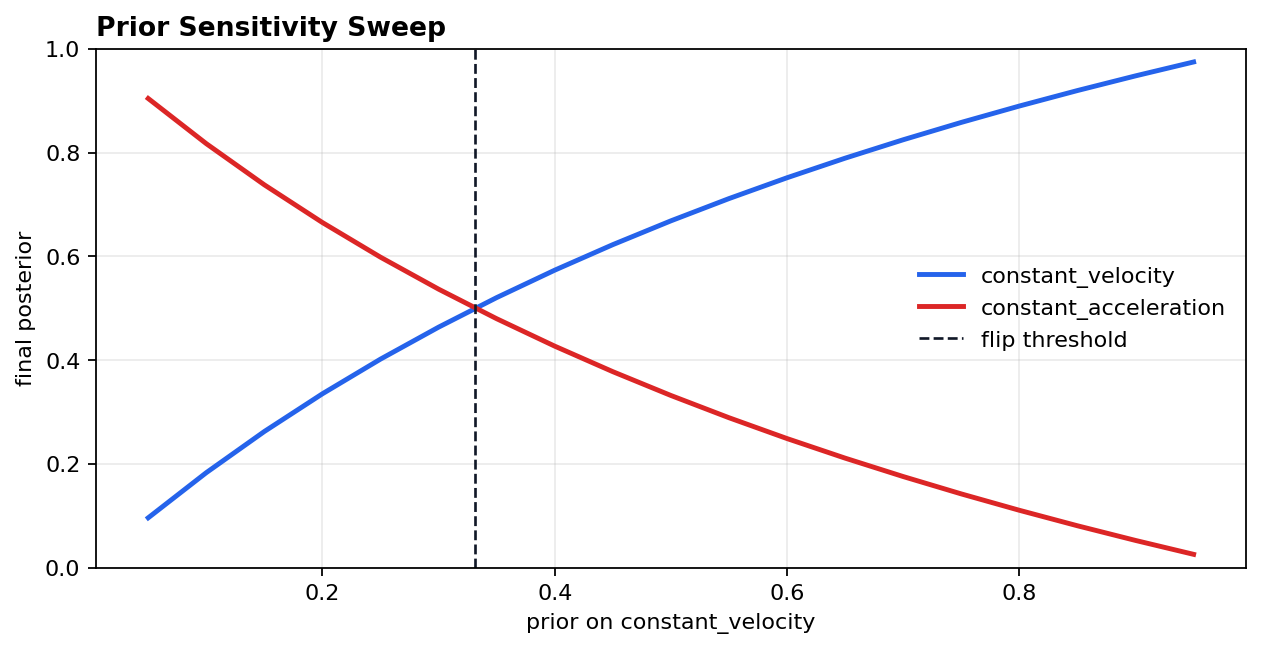
\includegraphics[width=0.9\textwidth]{prior_sweep_examples.png}
\caption{Representative prior-sweep examples from the Bayesian walkthrough suite.}
\end{figure}

\section{Corpus Adequacy-Driven Corpus Synthesis}
The corpus layer is treated as an optimization problem over balance, boundary coverage, feature excitation, leakage control, difficulty diversity, and nontriviality. The current automation does not simply audit the default corpus; it generates and ranks alternatives.
In symbolic form, one candidate corpus score takes the form
\begin{equation}
S_k = B_k + C_k + F_k + D_k - L_k - T_k - G_k,
\end{equation}
where the positive terms reward balance, boundary coverage, feature excitation, and difficulty diversity, while the negative terms penalize leakage, triviality, and degeneracy. This is the point where the repository moves beyond fixed toy datasets and starts reasoning about whether the data itself is good enough to trust later classifier conclusions.
\begin{enumerate}
  \item Load class definitions, scenario templates, and corpus adequacy objectives.
  \item Sample candidate corpus parameters over balance, difficulty, noise, outliers, and boundary emphasis.
  \item Generate a candidate corpus and extract the active feature sets.
  \item Audit adequacy, leakage, feature excitation, and quick oracle/classifier behavior.
  \item Score the corpus on balance, boundary coverage, feature excitation, difficulty diversity, and leakage penalties.
  \item Preserve both the selected candidate and the rejected or Pareto-front alternatives as evidence.
\end{enumerate}

\section{Automated Study Proposal and Promotion}
The repository now automatically generates study candidates from declared manifests and uses a validation ladder to issue \texttt{promote}, \texttt{revise}, \texttt{reject}, and \texttt{defer} decisions. The study-candidate layer is where corpus evidence, feature evidence, classifier compatibility, prior sensitivity, and implementation readiness are fused.
The current screening logic is intentionally two-stage. First, a static score \(Q_{\text{static}}\) screens candidate studies before they are expensive to evaluate. Second, executed common-study evidence provides a confirmation score \(Q_{\text{mc}}\). The current implementation therefore approximates
\begin{align}
Q_{\text{static}}
&=
\text{compatibility} + \text{separability} + \text{coverage} + \text{transfer}
\notag \\
&\quad - \text{dependency risk} - \text{history double-counting risk} - \text{prior fragility},
\end{align}
followed by
\begin{equation}
Q_{\text{mc}} = 0.60 \cdot \text{accuracy} + 0.25 \cdot (1 - \text{prior flip fraction}) + 0.15 \cdot (1 - \text{oracle gap}).
\end{equation}
The algorithmic skeleton used by the current implementation is:
\begin{enumerate}
  \item Load the current class-pair manifest, feature-set manifest, classifier manifest, and corpus objectives.
  \item Enumerate study candidates over $(\text{class pair}, \text{feature set}, \text{classifier}, \text{prior})$.
  \item Score each candidate statically for feature-class compatibility, oracle separability, corpus coverage, dimensional transfer, and double-counting risk.
  \item Reuse executed common-study evidence where available to attach classifier accuracy, prior sensitivity, and robustness signals.
  \item Emit \texttt{promote}, \texttt{revise}, \texttt{reject}, or \texttt{defer} according to the validation ladder rather than ad hoc manual judgment.
\end{enumerate}

\section{Feature and Class-Pair Analysis}
The methodology separates static identifiability from end-to-end classifier success. Feature-space overlap, oracle separability, pair difficulty, and duration/noise sensitivity are all treated as first-class evidence surfaces. This helps distinguish feature failure, corpus failure, and classifier failure.
If a class pair is hard, the repository does not immediately conclude that the classifier is weak. Instead it asks whether the feature layer has poor pairwise AUC, high overlap, weak excitation, or prior fragility. That separation of concerns is one of the main reasons the project can plausibly scale beyond one classifier family.

\begin{figure}[htbp]
\centering
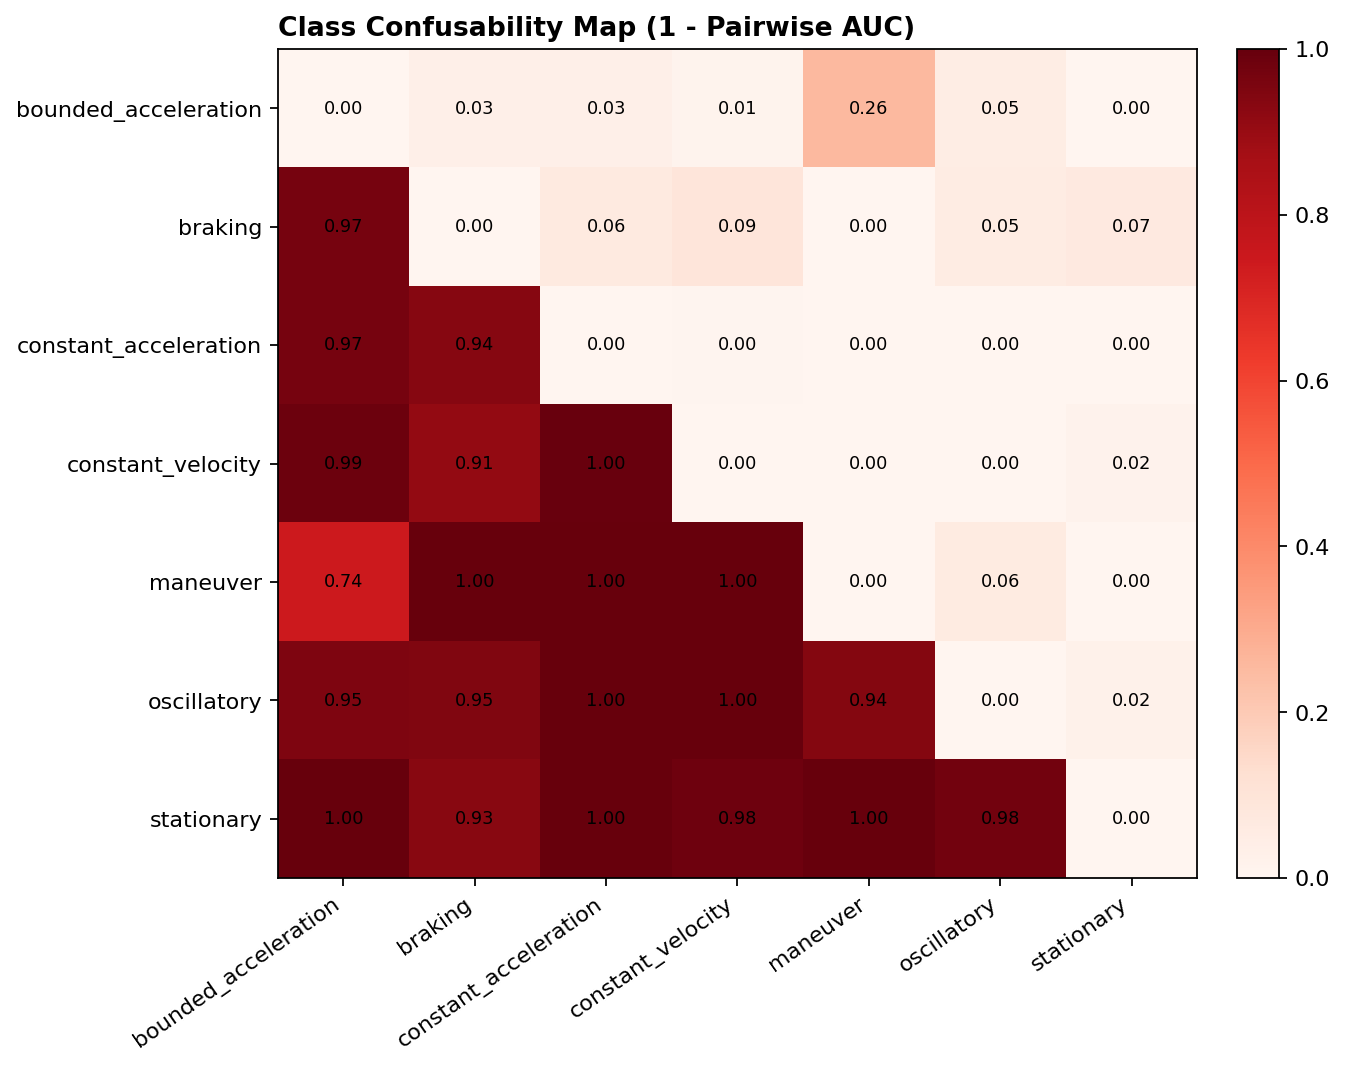
\includegraphics[width=0.9\textwidth]{class_confusability_heatmap.png}
\caption{Feature-space confusability remains pair-specific and motivates targeted feature or corpus work instead of one global leaderboard conclusion.}
\end{figure}

\section{From Generated Corpora To Promoted Studies}
The newer corpus-gym and study-candidate layers close the loop between data generation and methodology governance. In the current repository, objective-driven trajectory generation, quality-diversity archiving, backend-aware candidate generation, and validation-ladder promotion are all part of the same chain:
\begin{align}
\text{objective-driven trajectory proposals}
&\rightarrow
\text{generated corpus features}
\rightarrow
\text{classifier stress and prior sensitivity}
\notag \\
&\rightarrow
\text{study candidate generation}
\rightarrow
\text{validation ladder}
\rightarrow
d.
\end{align}
This is the architectural reason the disparate corpus, feature, and study docs belong together. They are not separate research threads anymore; they are stages of one methodology pipeline.

\section{Filtering Taxonomy and Advanced-Method Gates}
The current ladder proves the utility of pointwise, windowed, sequential Bayes, Kalman-bank, and transition-matrix evidence surfaces. It also records explicit no-go decisions for IMM, PF, and RBPF unless switching-mode or nonlinear evidence demands them. In the current decision reports, transition-aware accumulation is justified for switching witness problems, IMM remains decision-gated, PF remains decision-gated, and RBPF is only meaningful if future vector studies expose conditionally tractable mixed discrete/continuous structure.
The key policy claim is that advanced methods are downstream of failure evidence. If \(M_0\) is the current simpler method and \(M_1\) is a more advanced filter family, the repository is trying to justify a transition only when
\begin{equation}
\text{failure}(M_0, \mathcal{D}) \land \text{capability gain}(M_1) \land \text{measurable success criterion}(M_1)
\end{equation}
can all be stated explicitly. That is why the advanced-filter reports are decision artifacts rather than implementation plans by default.

\begin{figure}[htbp]
\centering
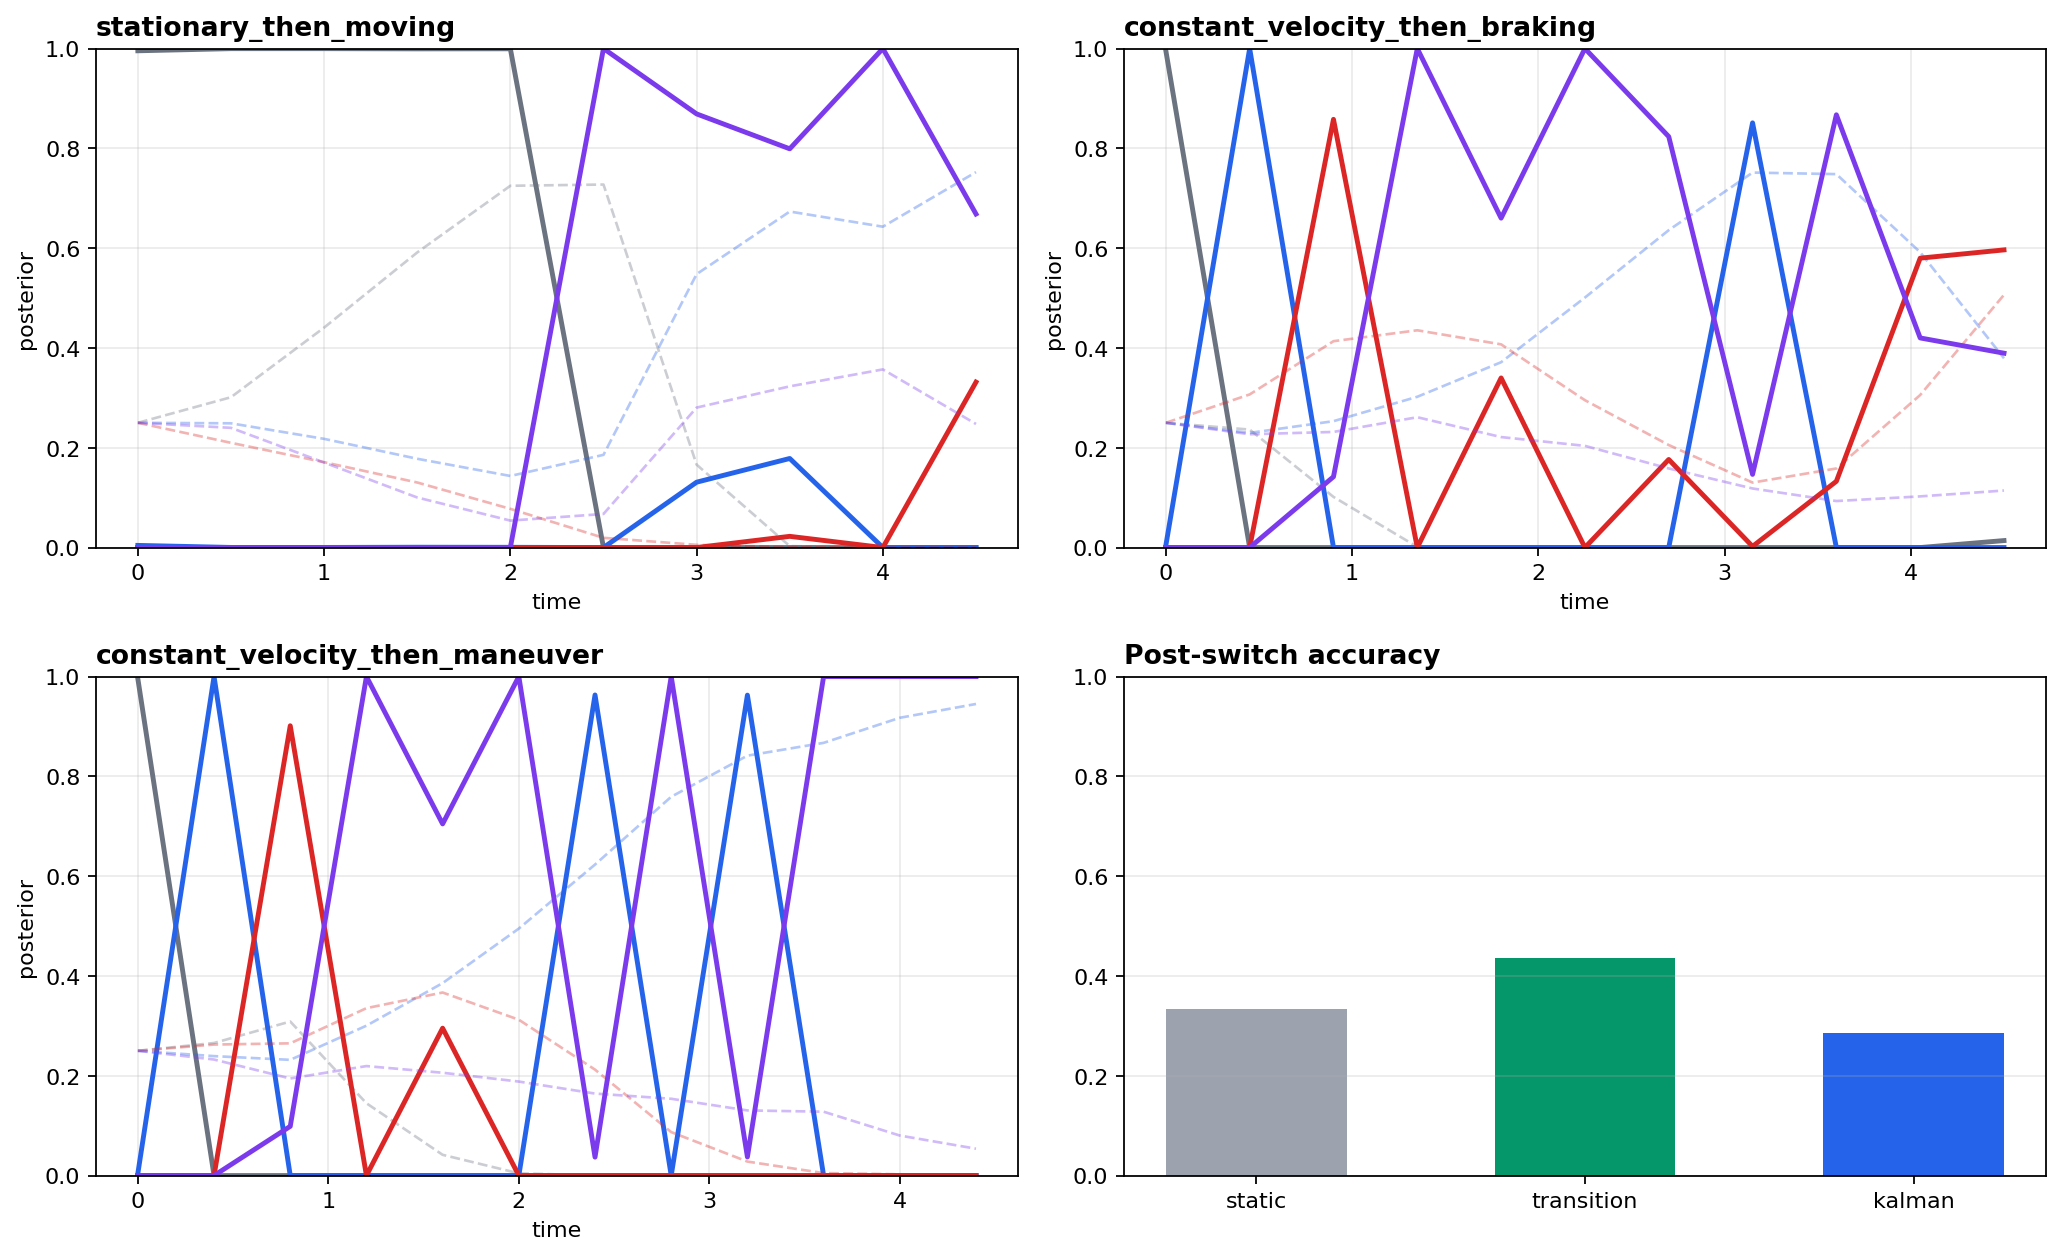
\includegraphics[width=0.9\textwidth]{transition_matrix_diagnostics.png}
\caption{Transition-matrix accumulation improves on static accumulation for switching trajectories and acts as the bridge evidence before considering IMM.}
\end{figure}

\section{Results Summary}
The current artifact stack proves the methodology process: study candidates can be declared, screened statically, evaluated against generated corpora, explained through posterior and prior-sensitivity surfaces, and assigned promotion decisions. It does not yet prove that the current synthetic corpus is final or fully adequate for every future class family. The strongest current claim is architectural rather than leaderboard-oriented: the repo can already express corpus design, feature analysis, evidence accumulation, evaluation, and promotion through shared artifacts.

\section{3D Transition Status}
The current methodology layer distinguishes three statuses: \texttt{dimension\_agnostic}, \texttt{adapter\_compatible}, and \texttt{rewrite\_required}. Contracts, shared evaluation, and study promotion are already dimension-aware. Scalar feature extraction and scalar state-space filtering remain rewrite-required, so current 3D readiness is methodological rather than dynamical.
The intended 3D lift is therefore not
\begin{equation}
\text{rewrite everything},
\end{equation}
but rather
\begin{equation}
\text{new corpus adapter} + \text{new feature geometry} + \text{new dynamics/measurement models} + \text{reuse of posterior/evaluation/reporting machinery}.
\end{equation}

\section{Limitations and Next Work}
The current common-study evidence still uses a class-score proxy for some walkthroughs, not a pure additive sensor likelihood decomposition for every family. The 1D studies are witness problems rather than a final deployment corpus. Some survey PDFs still contain cosmetic overfull-box warnings. The next work after this paper bundle is to integrate more numeric worked examples directly into the synthesis paper and then drive a true vector-valued corpus, feature, and filter lift through the same contracts proved here.

\end{document}
